% Preamble
\documentclass{beamer}
\usepackage[spanish]{babel}

% Packages
\usepackage{amsmath}
\usepackage[utf8]{inputenc}
\usepackage[T1]{fontenc}
\usepackage{graphicx}
\usepackage{algorithmicx}
\usepackage{algpseudocode}
\usepackage{caption}
\usepackage{courier}

\DeclareMathOperator{\atantwo}{atan2}

\captionsetup{justification=centering, font={scriptsize}, skip=0pt}

% Set bold vectors to satisfy requirements
\renewcommand\vec[1]{\ifstrequal{#1}{0}{\ensuremath{\mathbf{0}}}{\ensuremath{\boldsymbol{#1}}}}

\usetheme[compress]{Berlin}
\usecolortheme{wolverine}
\setbeamertemplate{page number in head/foot}[framenumber]
\setbeamercolor{institute in head/foot}{parent=palette primary}

\title[Dinámica molecular regida por el paso temporal]{Dinámica molecular regida por el paso temporal}
\subtitle{72.25 - Simulación de Sistemas}
\author[Flores Lucey, Llanos]{Alejo Flores Lucey\inst{1} \and Nehuén Gabriel Llanos\inst{2}}
\institute[Instituto Tecnológico de Buenos Aires]
{
    \inst{1}
    \href{mailto:afloreslucey@itba.edu.ar}{afloreslucey@itba.edu.ar}\\
    Legajo 62622
    \and
    \inst{2}
    \href{mailto:nllanos@itba.edu.ar}{nllanos@itba.edu.ar}\\
    Legajo 62511
}
\date{2024 1C | Grupo Nº3}
\titlegraphic{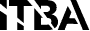
\includegraphics[height=0.5cm]{./itba}}

\makeatletter
\beamer@theme@subsectionfalse
\makeatother

\AtBeginSection[]{
    \begin{frame}
        \begin{beamercolorbox}[sep=8pt,center]{title}
            \usebeamerfont{title}\insertsection
        \end{beamercolorbox}
    \end{frame}
}

\begin{document}

    \begin{frame}
        \titlepage
    \end{frame}

    \section{Oscilador Puntual Amortiguado}

        \begin{frame}{Oscilador Puntual Amortiguado}
            \begin{itemize}
                \item Verlet Original
                \begin{equation*}
                    \begin{cases}
                        r(t + \Delta t) = 2 r(t) - r(t - \Delta t) + \Delta t^2 a(r(t), v(t))\\
                        r(t + \Delta t) = f(r(t), r(t - \Delta t), v(t))
                    \end{cases}
                \end{equation*}
                \begin{equation*}
                      \begin{cases}
                          v(t) = \frac{r(t + \Delta t) - r(t - \Delta t)}{2 \Delta t}\\
                          v(t) = g(r(t + \Delta t), r(t - \Delta t))
                      \end{cases}
                \end{equation*}
                \item Beeman
                \item Gear Predictor-Corrector
                \item Verlet 2.0 (se obtiene $r$ y $v$ para el mismo $\Delta t$.)
                \begin{equation*}
                    \begin{cases}
                        r(t + \Delta t) = f(r(t), r(t - \Delta t), v(t))\\
                        r(t + 2 \Delta t) = f(r(t + \Delta t), r(t), v(t))\\
                        v(t + \Delta t) = g(r(t + 2 \Delta t), r(t))
                    \end{cases}
                \end{equation*}
            \end{itemize}
        \end{frame}

        \begin{frame}{Oscilador Puntual Amortiguado: Resultados}
            \begin{figure}[H!]
                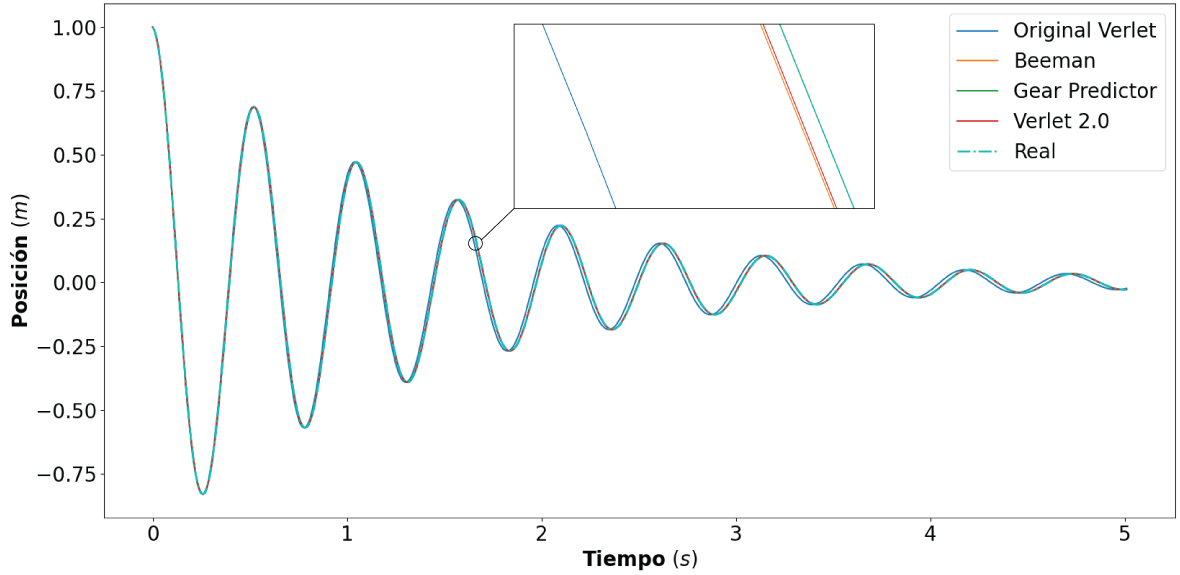
\includegraphics[width=0.9\textwidth]{./oscilador_resultados}
                \label{fig:oscilador_1}
            \end{figure}
        \end{frame}

        \begin{frame}{Oscilador Puntual Amortiguado: Error vs $\Delta t$}
            \begin{figure}[H!]
                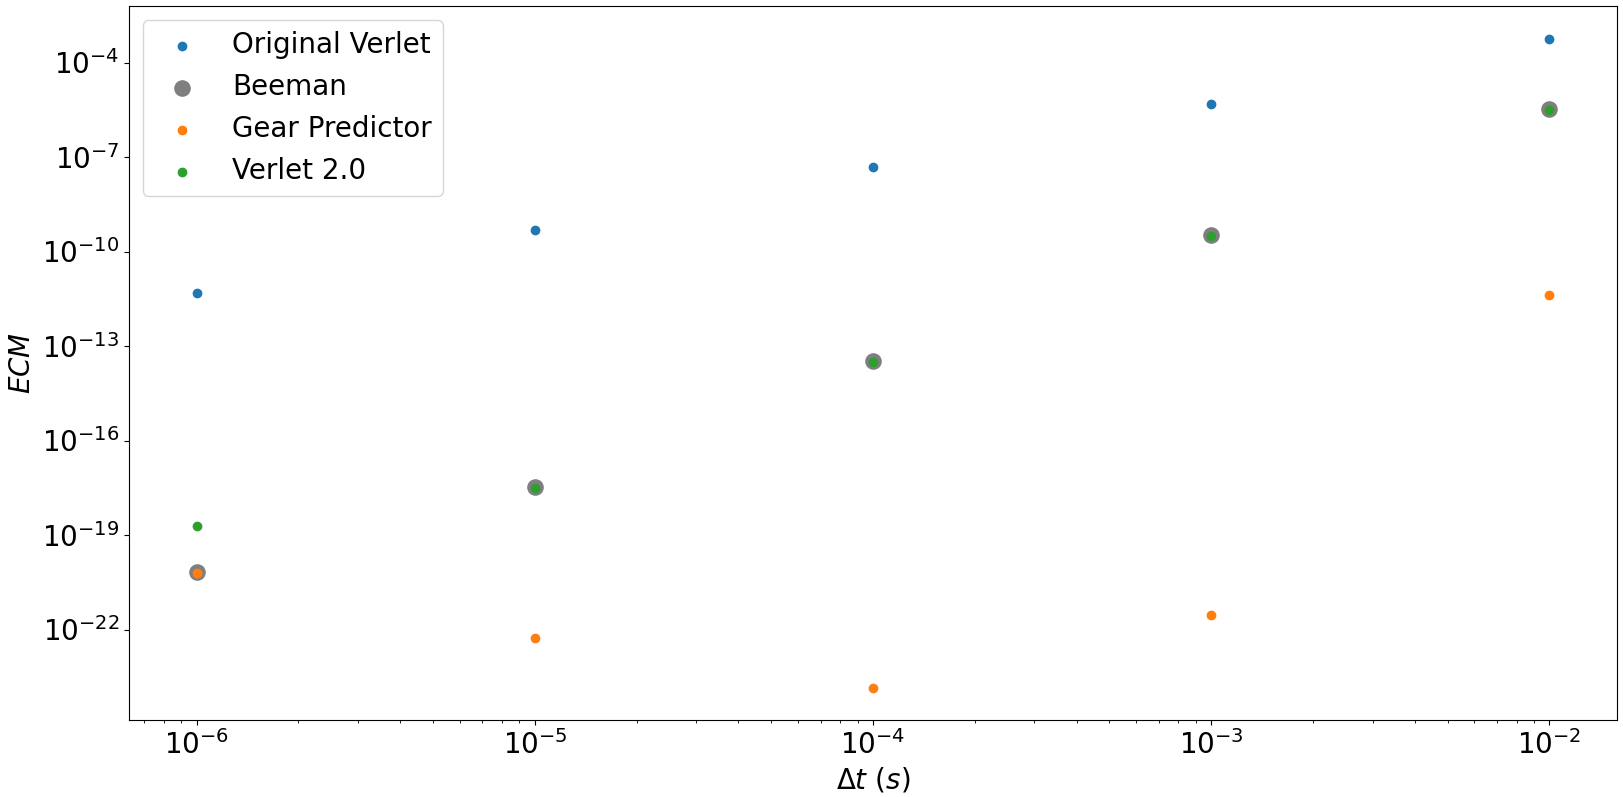
\includegraphics[width=0.9\textwidth]{./oscilador_error}
                \label{fig:oscilador_2}
            \end{figure}
        \end{frame}

    % HASTA ACA ESTÁ CAMBIADO

    \section{Introducción}

        \begin{frame}{Introducción}
            \begin{itemize}
                \item Dinámica molecular regida por el paso temporal.
                \item Simulación de un viaje espacial de una nave desde la Tierra a Marte en un espacio bidimensional.
                \item \textbf{Sistema real:}
                \begin{itemize}
                    \item El sistema solar.
                    \item Bolas de pool en una mesa de pool.
                    \item Deposición de un átomo en una superficie.
                \end{itemize}
            \end{itemize}
        \end{frame}

        \subsection{Fundamentos}

            \begin{frame}{Fundamentos}
                \begin{itemize}
                    \item Fuerza de gravedad entre dos planetas:
                        \begin{equation*}
                            \vec{F}_{p_1; p_2} = G \frac{m_p_1\ m_p_2}{r_{p_1;p_2}^2} \vec{e}_{p_1; p_2}
                        \end{equation*}
                    \item Constante de gravitación universal:
                        \begin{equation*}
                            G=6.6743 \times 10^{-20} \frac{km^3}{kg\ s^2}
                        \end{equation*}
                \end{itemize}
            \end{frame}

    \section{Implementación}

        \subsection{Arquitectura}

            \begin{frame}{Diagrama UML}
                \begin{figure}[htbp]
                    \centering
                    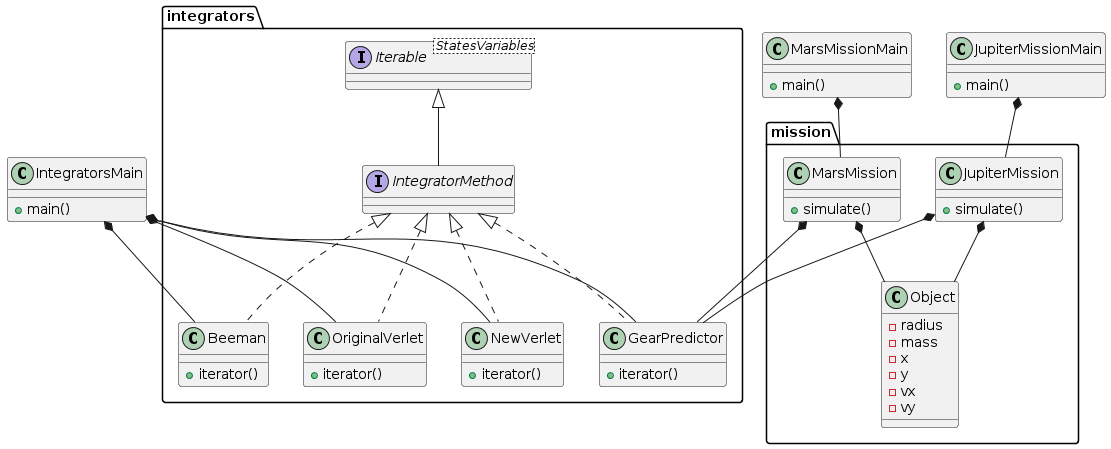
\includegraphics[width=\textwidth]{./architecture}
                    \label{fig:architecture}
                \end{figure}
            \end{frame}

        \subsection{Algoritmo}

            \begin{frame}{Pseudocódigo del algoritmo implementado}{}
                \begin{algorithmic}[1]
                    \ttfamily \scriptsize
                    \State Create output file
                    \State earthAcc $\gets$ [earthAccX, earthAccY](sun, mars)
                    \State marsAcc $\gets$ [marsAccX, marsAccY](sun, earth)
                    \State integrators $\gets$ [earthAcc, marsAcc]
                    \While{$t < departureTime + twoYears$}
                        \If{$t = departureTime$}
                            \State earthAcc $\gets$ [earthAccX, earthAccY](sun, mars, ship)
                            \State marsAcc $\gets$ [marsAccX, marsAccY](sun, earth, ship)
                            \State shipAcc $\gets$ [shipAccX, shipAccY](sun, earth, mars)
                            \State integrators $\gets$ [earthAcc, marsAcc, shipAcc]
                        \EndIf
                        \State \Call{UpdateStateVariables}{earth}
                        \State \Call{UpdateStateVariables}{mars}
                        \If{$t \geq departureTime$}
                            \State \Call{UpdateStateVariables}{ship}
                        \EndIf
                        \State \Call{WriteOutput}{earth, mars, ship}
                        \State $i \gets i + dt$
                    \EndWhile
                \end{algorithmic}
            \end{frame}

    \section{Simulaciones}

        \subsection{Parámetros de entrada}

            \begin{frame}{Parámetros de entrada}
                \begin{itemize}
                    \item Parámetros de entrada fijos:
                    \begin{itemize}
                        \item $m_{sun}$: \alert{$2\times 10^{30}kg$}
                        \item $R_{sun}$: \alert{$696340km$}
                        \item $m_{earth}$: \alert{$5,9722\times 10^{24}kg$}
                        \item $R_{earth}$: \alert{$6371km$}
                        \item $\vec{r}_{earth}$: \alert{$(-1,219\times 10^{8}; -8,831\times 10^{7})km$}
                        \item $\vec{v}_{earth}$: \alert{$(1,698\times 10; -2,423\times 10)km/s$}
                        \item $m_{mars}$: \alert{$6,4\times 10^{23}kg$}
                        \item $R_{mars}$: \alert{$3389,5km$}
                        \item $\vec{r}_{mars}$: \alert{$(1,758\times 10^{8}; -1,087\times 10^{8})km$}
                        \item $\vec{v}_{mars}$: \alert{$(1,366; 2,268)km/s$}
                        \item $m_{ship}$: \alert{$2\times 10^{5} kg$}
                        \item $d_{shipRelEarth}$: \alert{$1500km$}
                    \end{itemize}
                    \item Parámetros de entrada variables:
                    \begin{itemize}
                        \item $v_{shipTangRelEarth}$: \alert{$\{15,02; 15,021; ...; 15,219; 15,22\}km/s$}
                        \item ${dt}$: \alert{$\{0,01;0,1;1;10;100;1000;10000\}s$}
                    \end{itemize}
                \end{itemize}
            \end{frame}

        \subsection{Observables}

            \begin{frame}{Conservación de la Energía en el sistema}
                \begin{itemize}
                    \item Energía Cinética:
                    \begin{equation*}
                        K_{p} = \frac{1}{2} m_{p} v_{p}^2
                    \end{equation*}
                    \item Energía Potencial:
                    \begin{equation*}
                        U_{(p_1,p_2)} = - G \left( \frac{m_{p_1} m_{p_2}}{\sqrt{(x_{p_1} - x_{p_2})^2 + (y_{p_1} - y_{p_2})^2}} \right)
                    \end{equation*}
                    \item Conservación de la Energía en el sistema:
                    \begin{equation*}
                        K_{total} + U_{total} = \text{constante}
                    \end{equation*}
                \end{itemize}
            \end{frame}

            \begin{frame}{Momento de partida de la nave para llegar a Marte}
                \begin{itemize}
                    \item 730 lanzamientos (1 por día). Obtenemos día que logra distancia mínima.
                    \item 48 lanzamientos (1 por hora) para el día obtenido y el anterior. Obtenemos hora que logra distancia mínima.
                    \item 120 lanzamientos (1 por minuto) para la hora obtenida y la anterior. Obtenemos minuto que logra distancia mínima.
                    \item Distancia entre la nave y marte:
                    \begin{equation*}
                        d_{(ship, mars)} = \sqrt{(x_{ship} - x_{mars})^2 + (y_{ship} - y_{mars})^2}
                    \end{equation*}
                \end{itemize}
            \end{frame}

            \begin{frame}{Variación módulo de velocidad de la nave para llegar a Marte}
                \begin{itemize}
                    \item Obtenemos la velocidad de la nave en coordenadas cartesianas.
                    \begin{minipage}[t]{0.55\textwidth}
                        \begin{equation*}
                            \hat{e_n} = \frac{\vec{r}_{ship} - \vec{r}_{earth}}{||\vec{r}_{ship} - \vec{r}_{earth}||}= (e_n \hat{\imath}, e_n \hat{\jmath})
                        \end{equation*}
                    \end{minipage}
                    \hfill
                    \begin{minipage}[t]{0.3\textwidth}
                        \begin{equation*}
                            \hat{e_t} = (-e_n \hat{\imath}, e_n \hat{\jmath})
                        \end{equation*}
                    \end{minipage}
                    \begin{equation*}
                        \vec{v}_{x_{ship}} = \vec{v}_{x_{earth}} + v_{shipTangRelEarth} \cdot e_t \hat{\imath}
                    \end{equation*}
                    \begin{equation*}
                        \vec{v}_{y_{ship}} = \vec{v}_{y_{earth}} +v_{shipTangRelEarth} \cdot e_t \hat{\jmath}
                    \end{equation*}
                    \begin{equation*}
                        v_{shipTangRelEarth} = 7,12km/s + \alpha
                    \end{equation*}
                    \begin{equation*}
                        \alpha \in \{7,9;7,901;...;8,099;8,1\}km/s
                    \end{equation*}
                \end{itemize}
            \end{frame}

            \begin{frame}{Misión Júpiter}
                \begin{itemize}
                    \item Se agrega el planeta Júpiter al sistema.
                    \item La órbita de Júpiter es de 12 años, pero se simulan 5 dado que existe un patrón.
                    \item Se realiza el mismo análisis que para el viaje a Marte.
                    \item Parámetros fijos:
                    \begin{itemize}
                        \item $m_{jupiter}$: \alert{$1,898\times 10^{27}kg$}
                        \item $R_{jupiter}$: \alert{$69911km$}
                        \item $\vec{r}_{jupiter}$: \alert{$(4,197\times 10^{8}; 6,209\times 10^{8})km$}
                        \item $\vec{v}_{jupiter}$: \alert{$(-1,098\times 10; 7,940)km/s$}
                    \end{itemize}
                \end{itemize}
            \end{frame}

    \section{Resultados}

        \subsection{Animación del sistema}

            \begin{frame}{Animación del sistema}{}
                \vspace*{-0.3cm}
                \begin{minipage}[t]{0.49\textwidth}
                    \begin{figure}[H!]
                        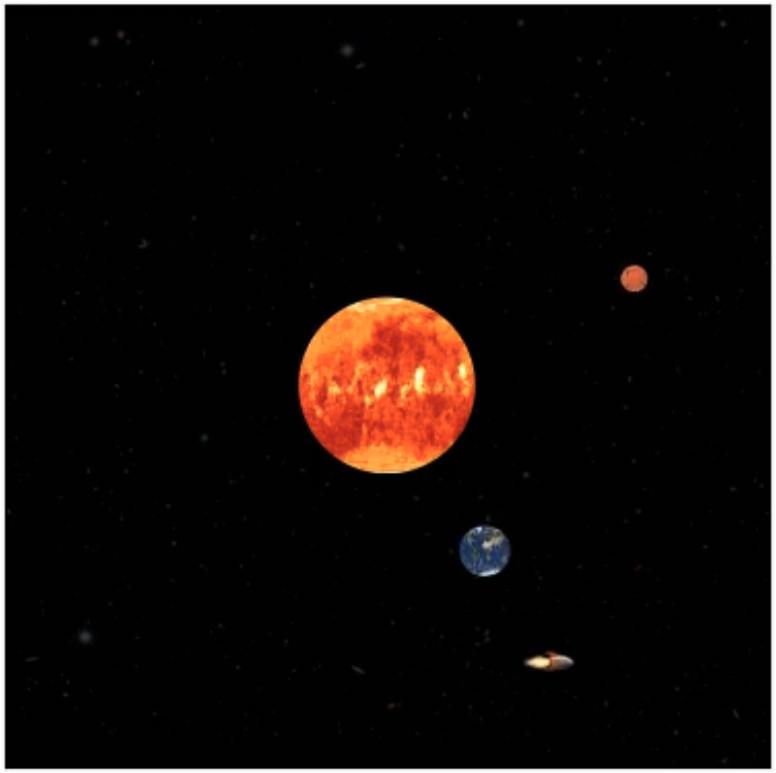
\includegraphics[width=\textwidth]{./animacion_marte_1}
                        \caption*{Véase la animación completa en \url{https://youtu.be/1PgQa7WLQ6g}.}
                        \label{fig:marte_1}
                    \end{figure}
                    \vspace*{-0.5cm}
                    \begin{beamercolorbox}[sep=5pt,center]{block body}
                        \centering
                        \small{Día de partida: 0}
                    \end{beamercolorbox}
                \end{minipage}
                \hfill
                \begin{minipage}[t]{0.49\textwidth}
                    \begin{figure}[H!]
                        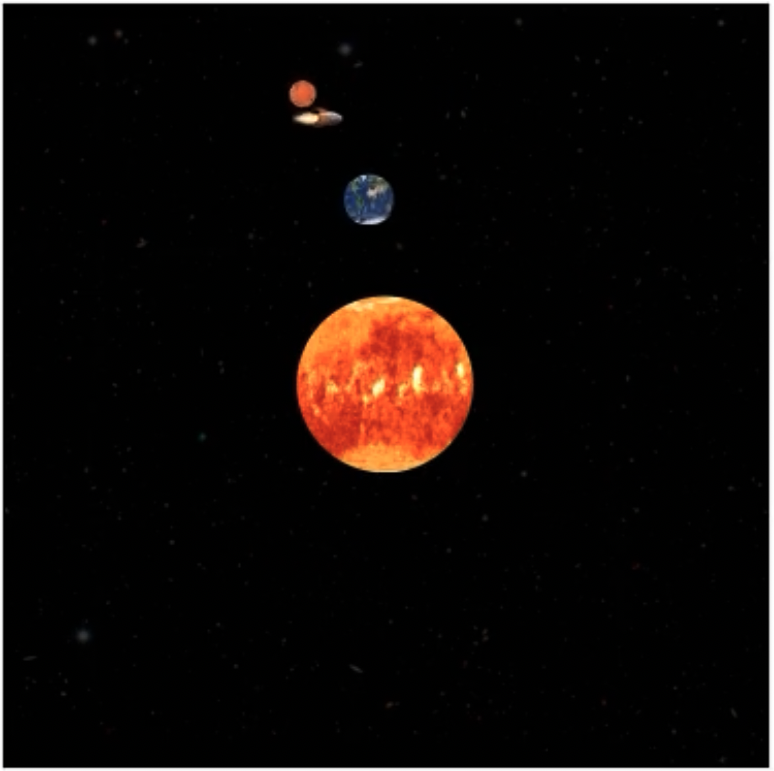
\includegraphics[width=\textwidth]{./animacion_marte_2}
                        \caption*{Véase la animación completa en \url{https://youtu.be/MAS-4i-Jz9Q}.}
                        \label{fig:marte_2}
                    \end{figure}
                    \vspace*{-0.5cm}
                    \begin{beamercolorbox}[sep=5pt,center]{block body}
                        \centering
                        \small{Día de partida: 172}
                    \end{beamercolorbox}
                \end{minipage}
            \end{frame}

        \subsection{Elección del $\Delta t$}

            \begin{frame}{Energía perdida en función del tiempo}{Elección del $\Delta t$}
                    \begin{figure}[H!]
                        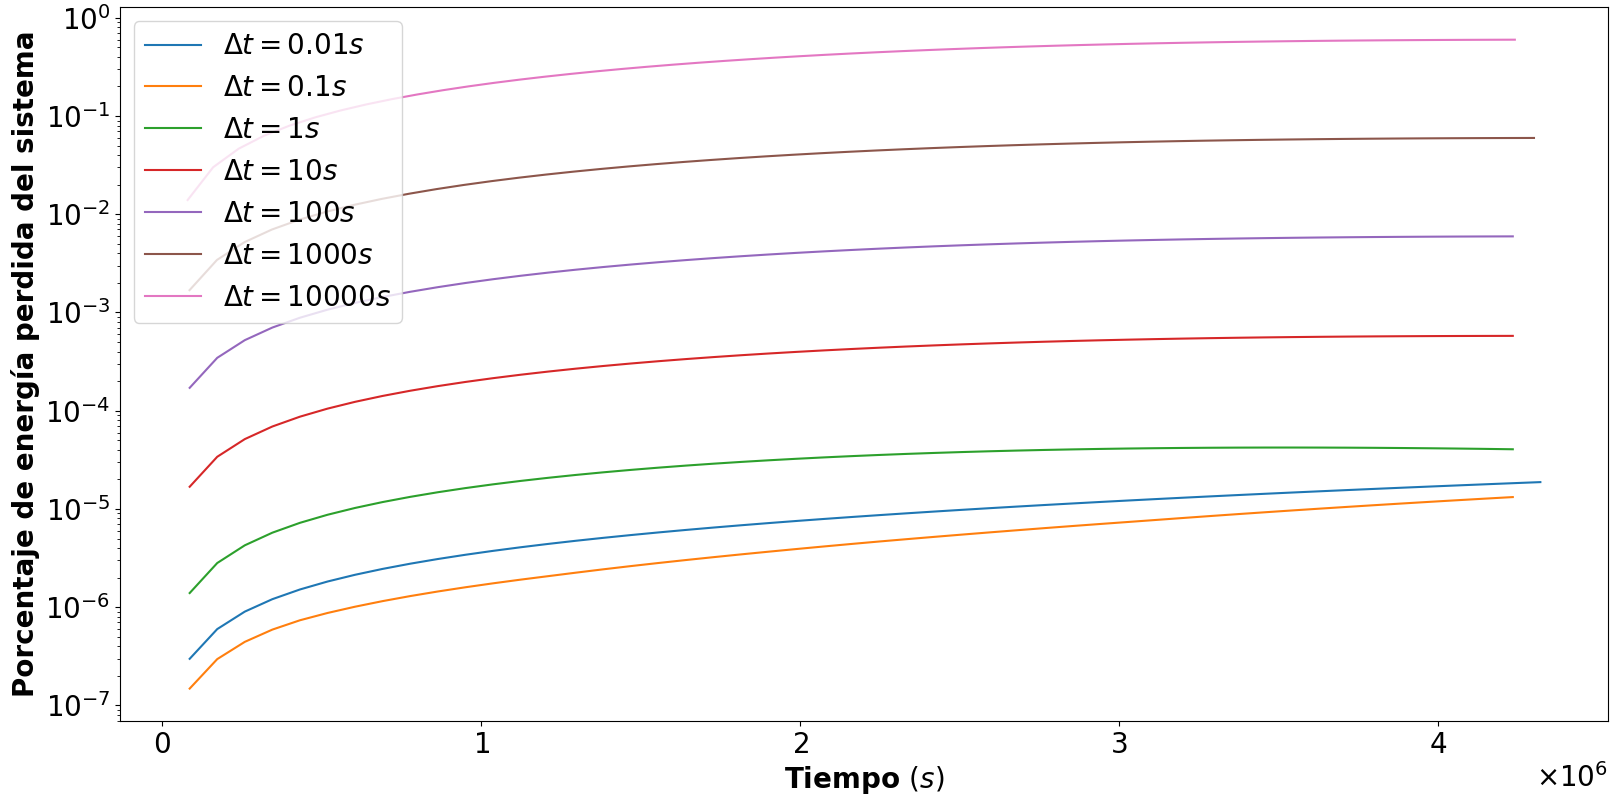
\includegraphics[width=0.9\textwidth]{./energia_perdida_vs_tiempo}
                        \label{fig:marte_3}
                    \end{figure}
                    \begin{beamercolorbox}[sep=5pt,center]{block body}
                        \centering
                        \small{Estudio en 50 días}
                    \end{beamercolorbox}
            \end{frame}

            \begin{frame}{Promedio de energía perdida vs $\Delta t$}{Elección del $\Delta t$}
                \begin{figure}[H!]
                    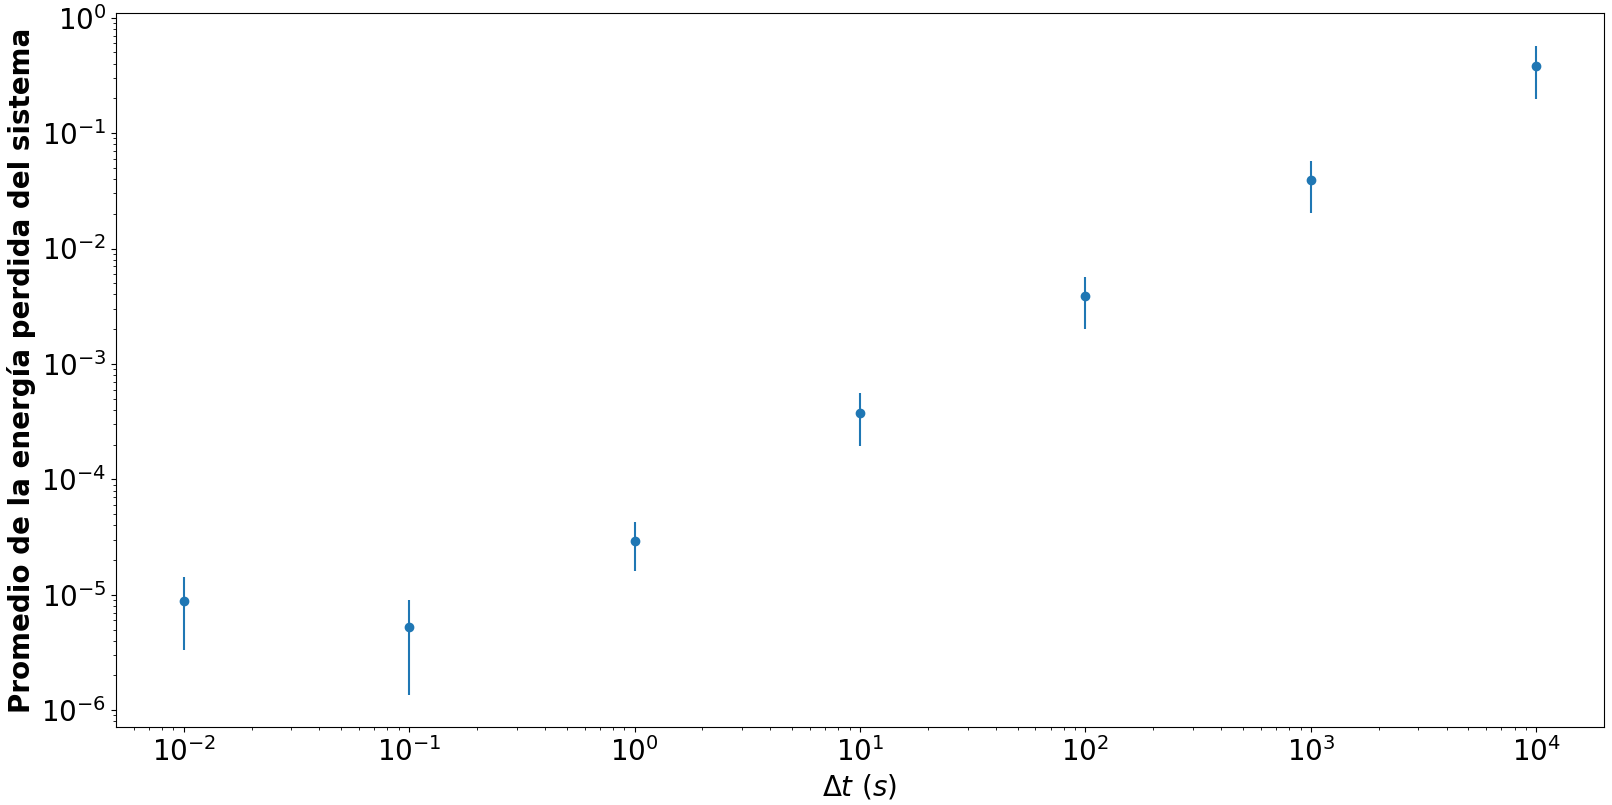
\includegraphics[width=0.9\textwidth]{./promedio_energia_perdida_vs_dt}
                    \label{fig:marte_4}
                \end{figure}
                \begin{beamercolorbox}[sep=5pt,center]{block body}
                    \centering
                    \small{Estudio en 50 días}
                \end{beamercolorbox}
            \end{frame}

        \subsection{Momento óptimo de partida para arribar a Marte}

            \begin{frame}{Distancia mínima a Marte vs día de partida}{Momento óptimo de partida para arribar a Marte}
                \begin{figure}[H!]
                    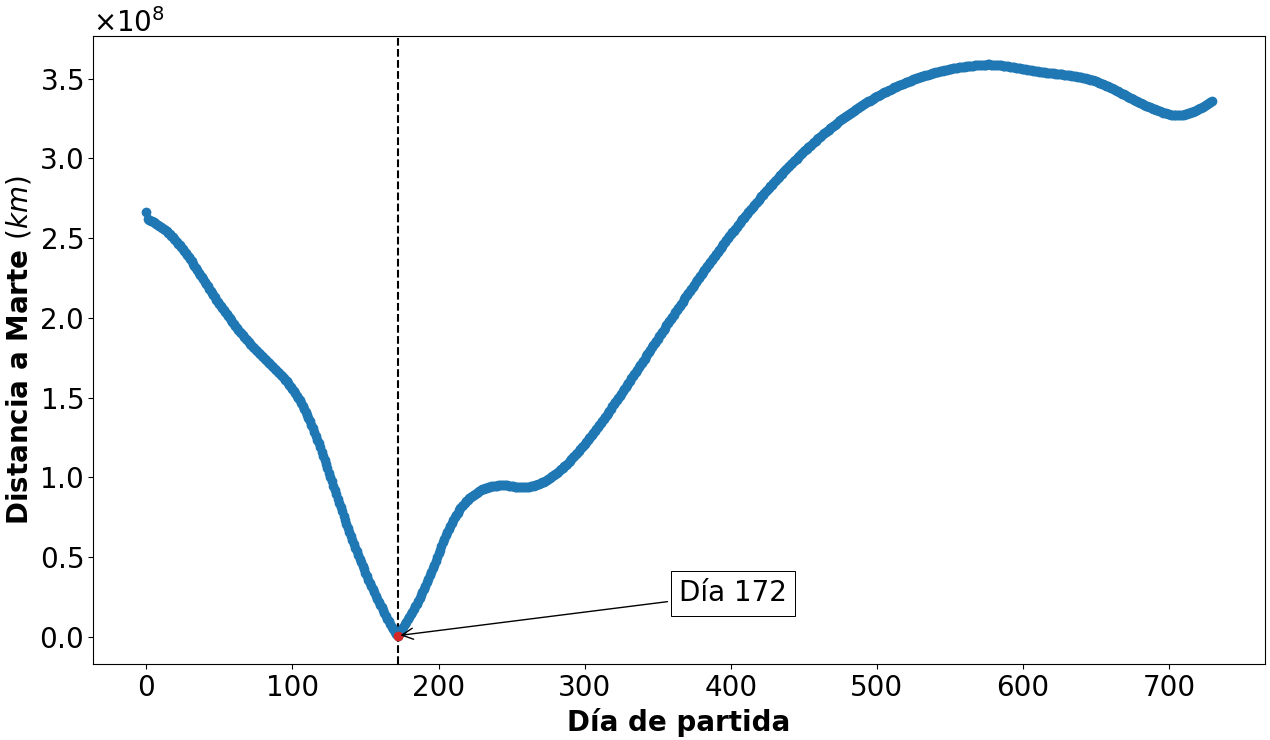
\includegraphics[width=0.9\textwidth]{./distancia_a_marte_vs_dia_de_partida}
                    \label{fig:marte_5}
                \end{figure}
                \begin{beamercolorbox}[sep=5pt,center]{block body}
                    \centering
                    \small{$\Delta t = 60s$ ; Misión exitosa si $d_{nave-marte} < 3520 km$}
                \end{beamercolorbox}
            \end{frame}

            \begin{frame}{Distancia mínima a Marte vs hora de partida}{Momento óptimo de partida para arribar a Marte. A partir de 171d}
                \begin{figure}[H!]
                    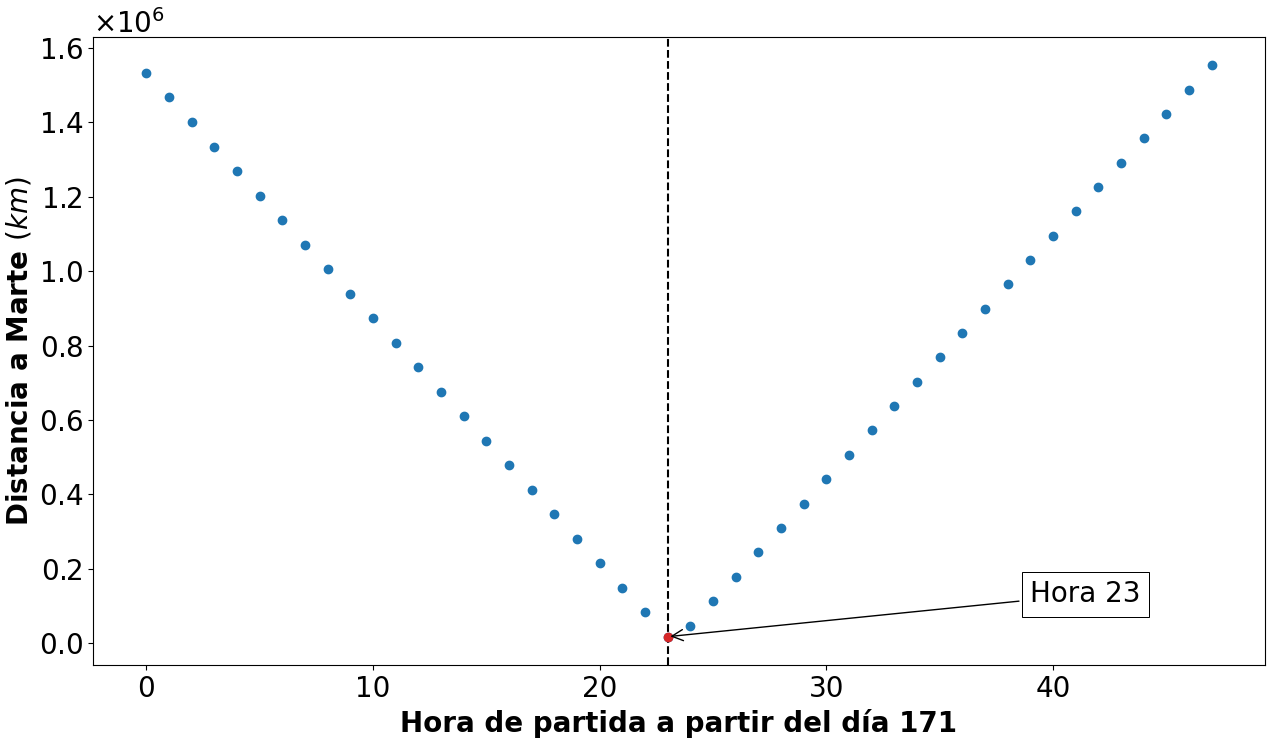
\includegraphics[width=0.9\textwidth]{./distancia_a_marte_vs_hora_de_partida}
                    \label{fig:marte_6}
                \end{figure}
                \begin{beamercolorbox}[sep=5pt,center]{block body}
                    \centering
                    \small{$\Delta t = 60s$ ; Misión exitosa si $d_{nave-marte} < 3520 km$}
                \end{beamercolorbox}
            \end{frame}

            \begin{frame}{Distancia mínima a Marte vs minuto de partida}{Momento óptimo de partida para arribar a Marte. A partir de 171d 22h}
                \begin{figure}[H!]
                    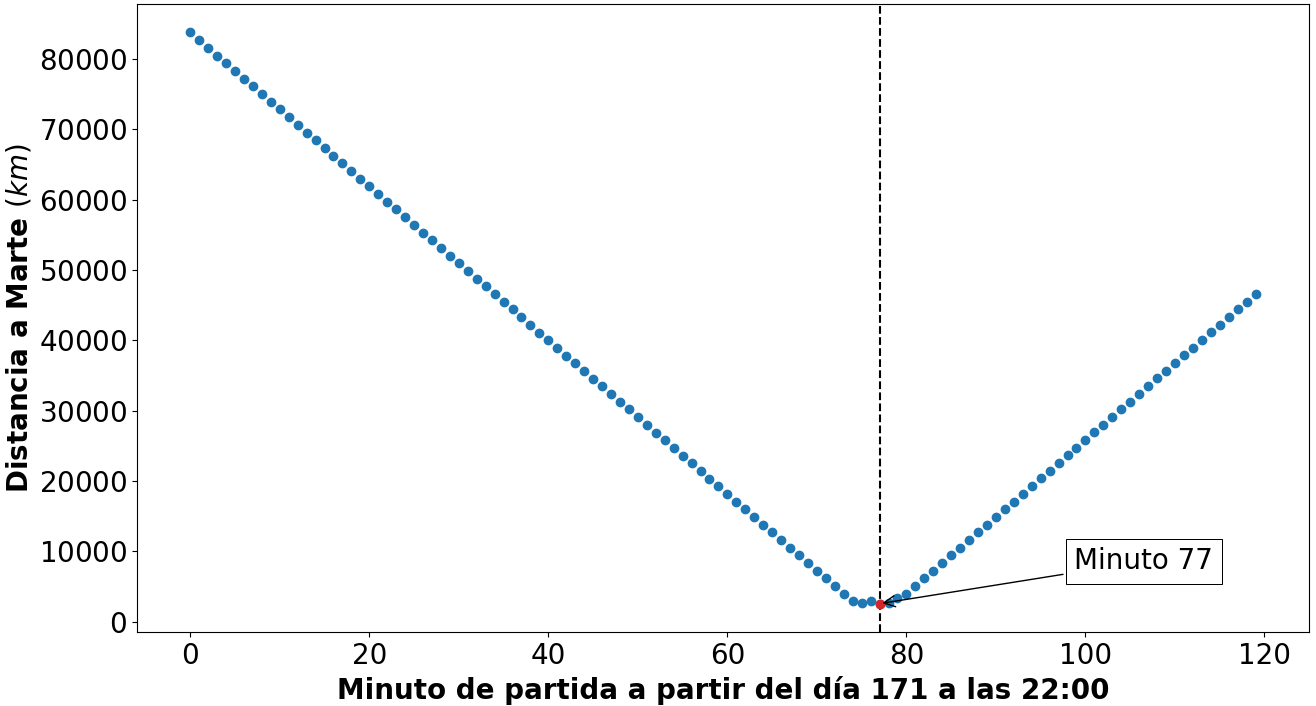
\includegraphics[width=0.9\textwidth]{./distancia_a_marte_vs_minuto_de_partida}
                    \label{fig:marte_7}
                \end{figure}
                \begin{beamercolorbox}[sep=5pt,center]{block body}
                    \centering
                    \small{$\Delta t = 60s$ ; $d_{nave-marte} = 2547.98 km$}
                \end{beamercolorbox}
            \end{frame}

        \subsection{Velocidad de la nave vs tiempo}

            \begin{frame}{Módulo de la velocidad de la nave vs tiempo}{Partida de la nave: 171d 23h 17m}
                \begin{figure}[H!]
                    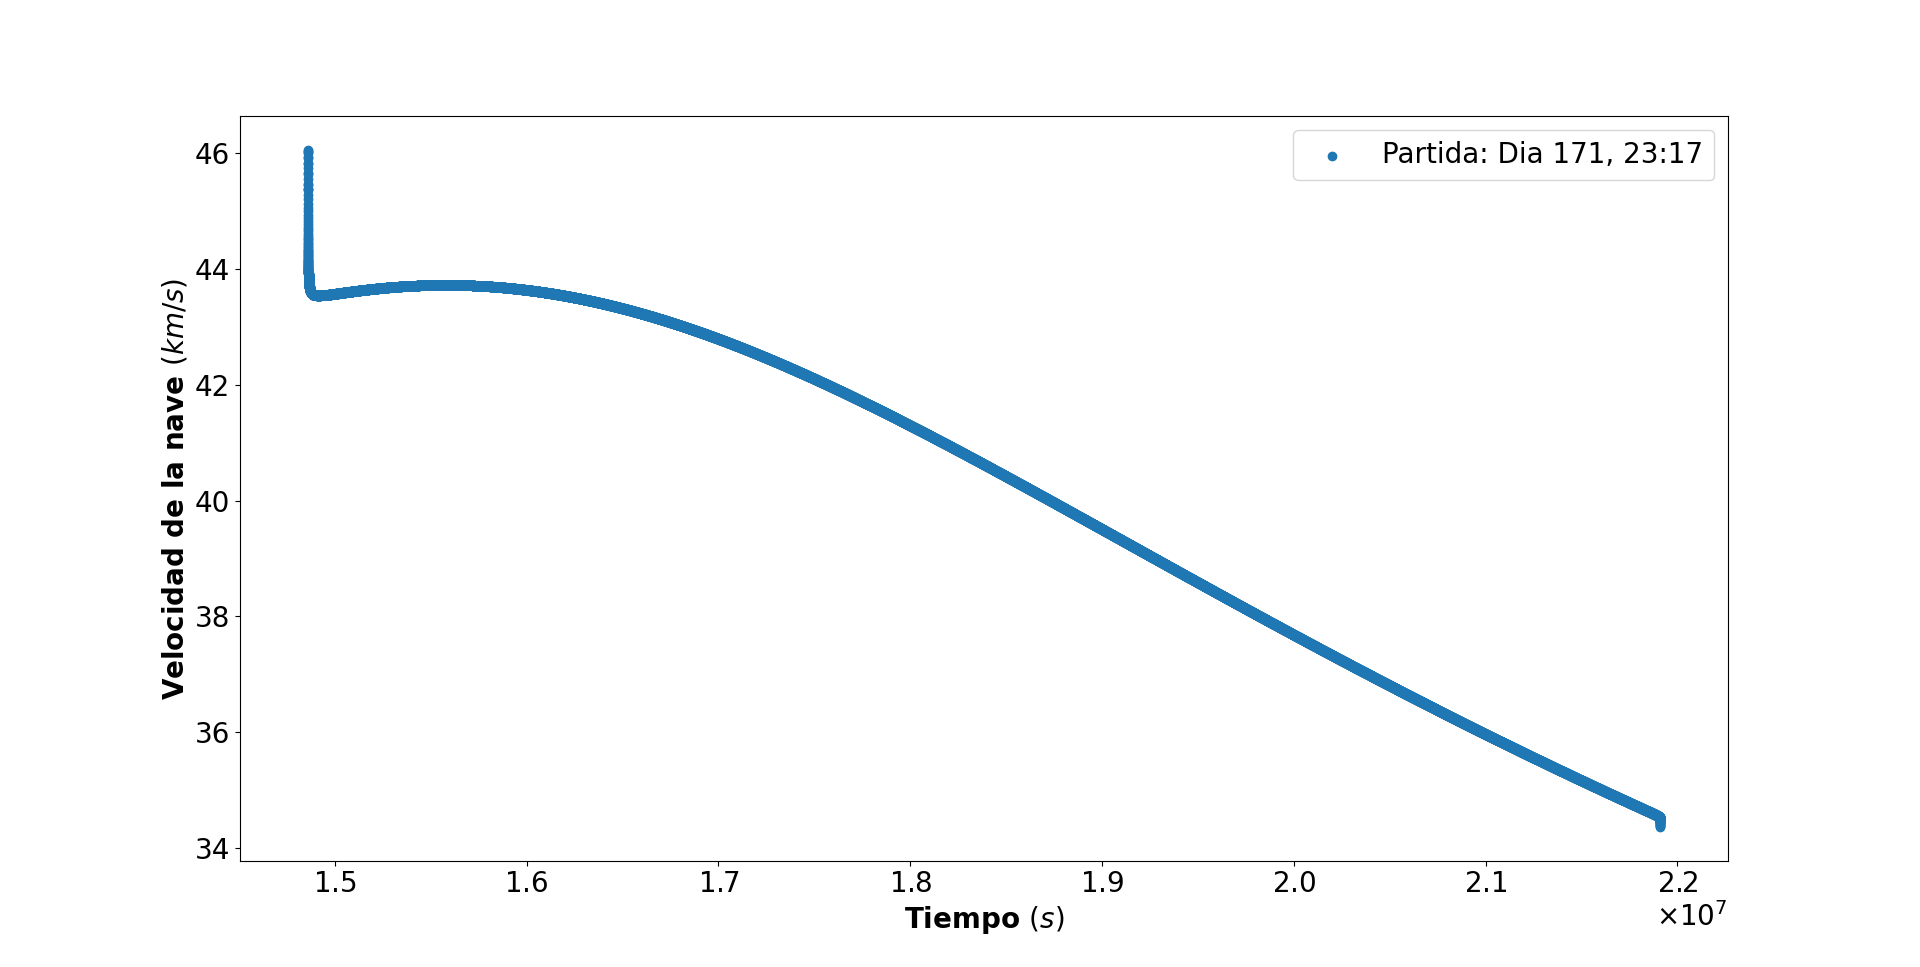
\includegraphics[width=0.9\textwidth]{./velocity_vs_time_for_travel_to_mars}
                    \label{fig:marte_8}
                \end{figure}
                \begin{beamercolorbox}[sep=5pt,center]{block body}
                    \centering
                    \small{$\Delta t = 60s$ ; $t_{vuelo} = 81d 15h 5m$}
                \end{beamercolorbox}
            \end{frame}

        \subsection{Variación de la velocidad incial de la nave}

            \begin{frame}{Distancia mínima a Marte vs velocidad inicial de la nave}{Partida de la nave: 171d 23h 17m}
                \begin{figure}[H!]
                    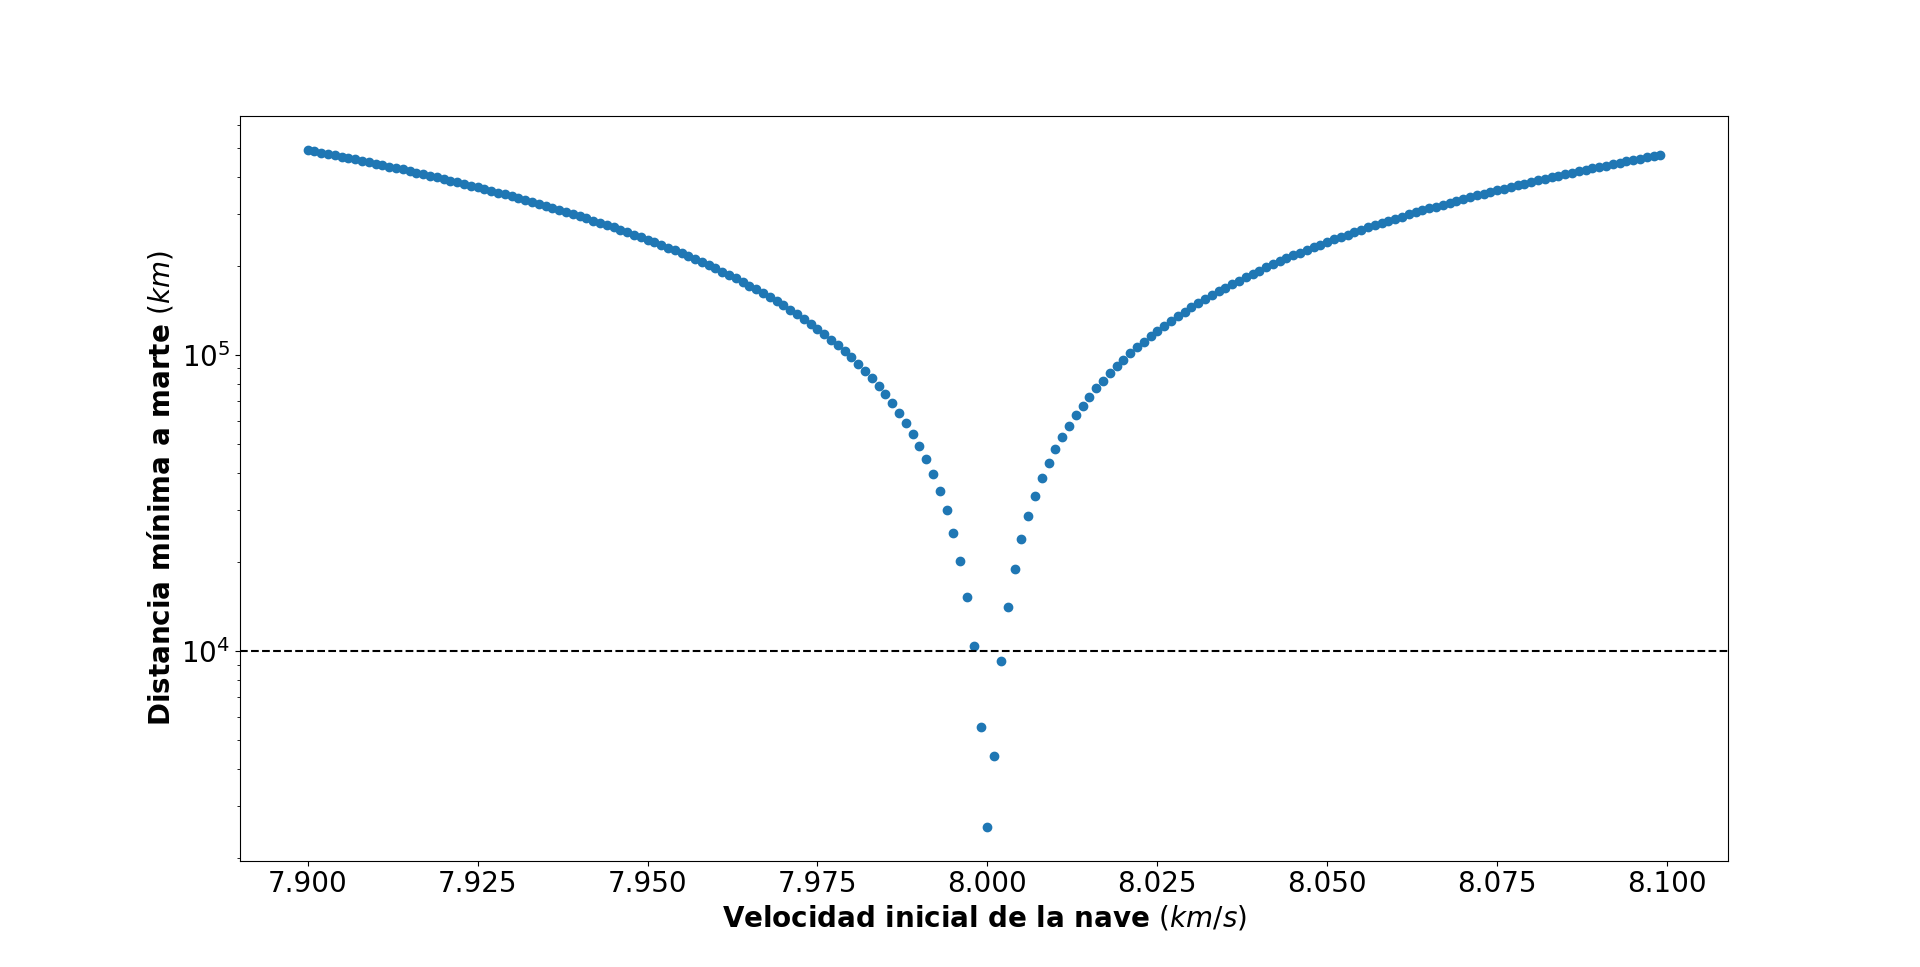
\includegraphics[width=0.9\textwidth]{./min_distance_vs_v0_logaritmica_line_in_10^4_scatter}
                    \label{fig:marte_9}
                \end{figure}
                \begin{beamercolorbox}[sep=5pt,center]{block body}
                    \centering
                    \small{$\Delta t = 60s$ ; Misión exitosa si $d_{nave-marte} < 10^4 km$}
                \end{beamercolorbox}
            \end{frame}

            \begin{frame}{Distancia mínima a Marte vs velocidad inicial de la nave}{Partida de la nave: 171d 23h 17m}
                \begin{figure}[H!]
                    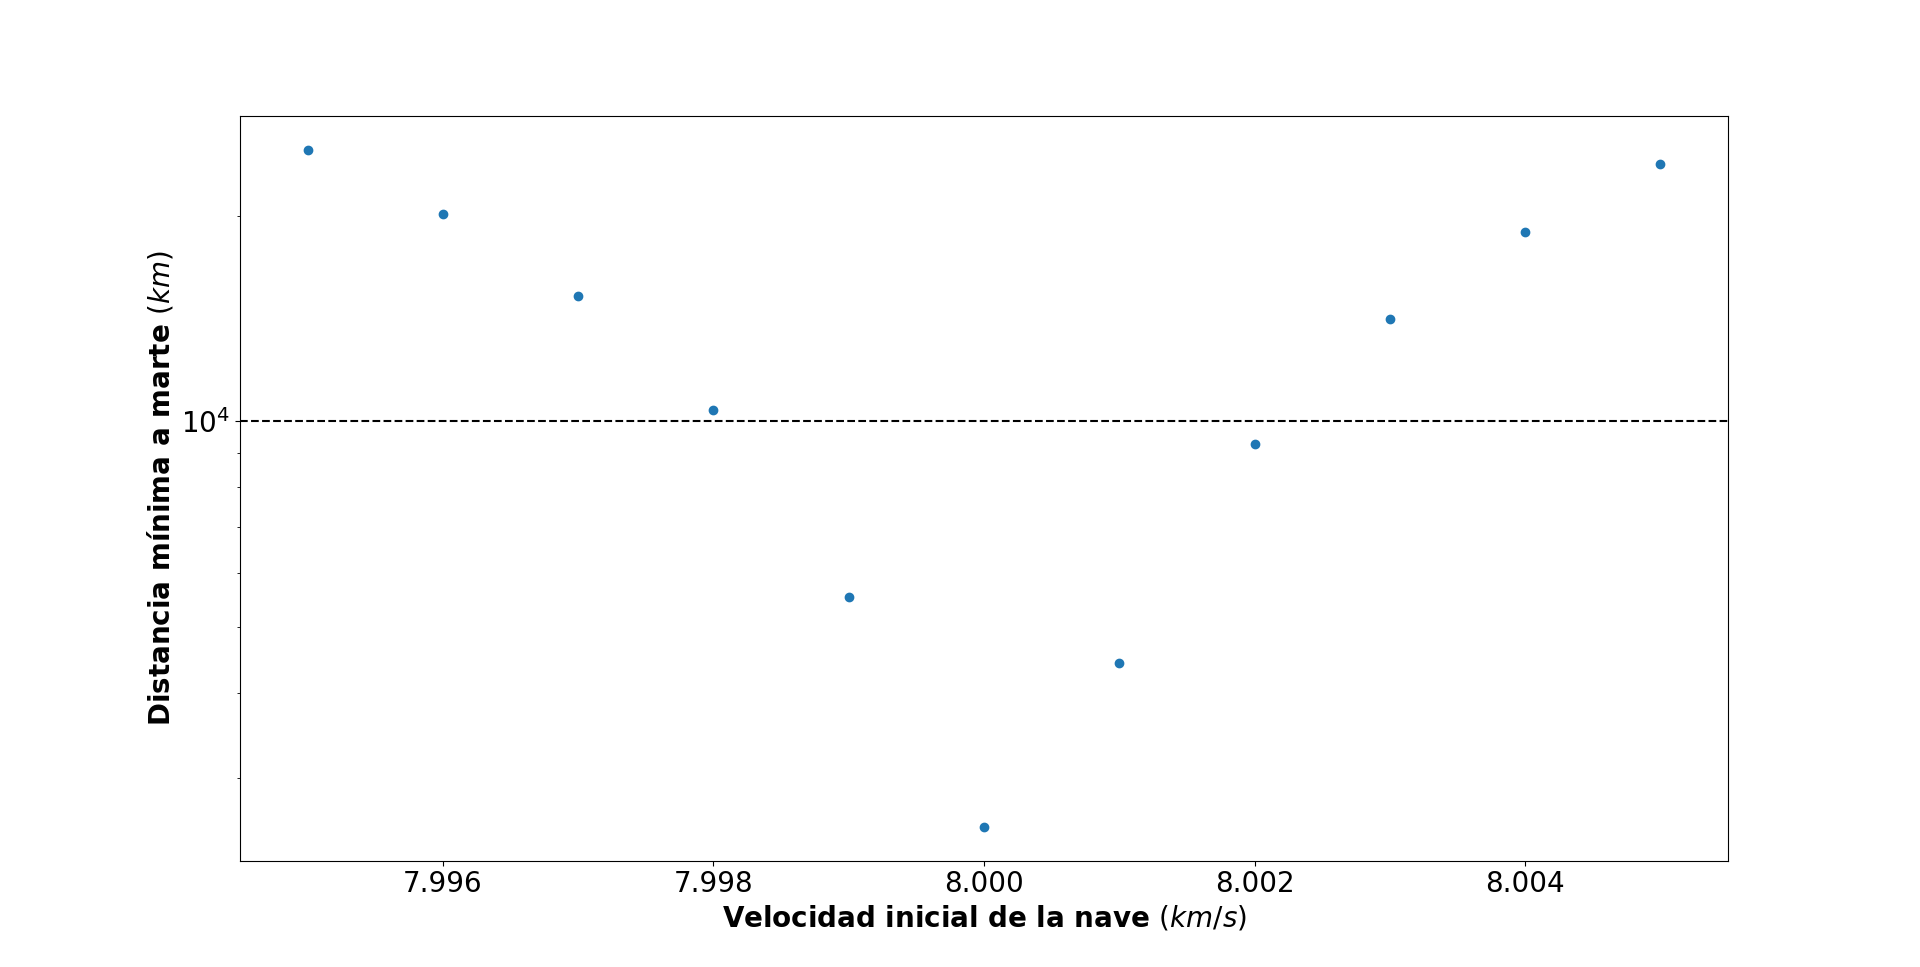
\includegraphics[width=0.9\textwidth]{./min_distance_vs_v0_logaritmica_line_in_10^4_reduced_scatter}
                    \label{fig:marte_10}
                \end{figure}
                \begin{beamercolorbox}[sep=5pt,center]{block body}
                    \centering
                    \small{$\Delta t = 60s$ ; Misión exitosa si $d_{nave-marte} < 10^4 km$}
                \end{beamercolorbox}
            \end{frame}

            \begin{frame}{Tiempo de vuelo vs velocidad inicial de la nave}{Partida de la nave: 171d 23h 17m}
                \begin{figure}[H!]
                    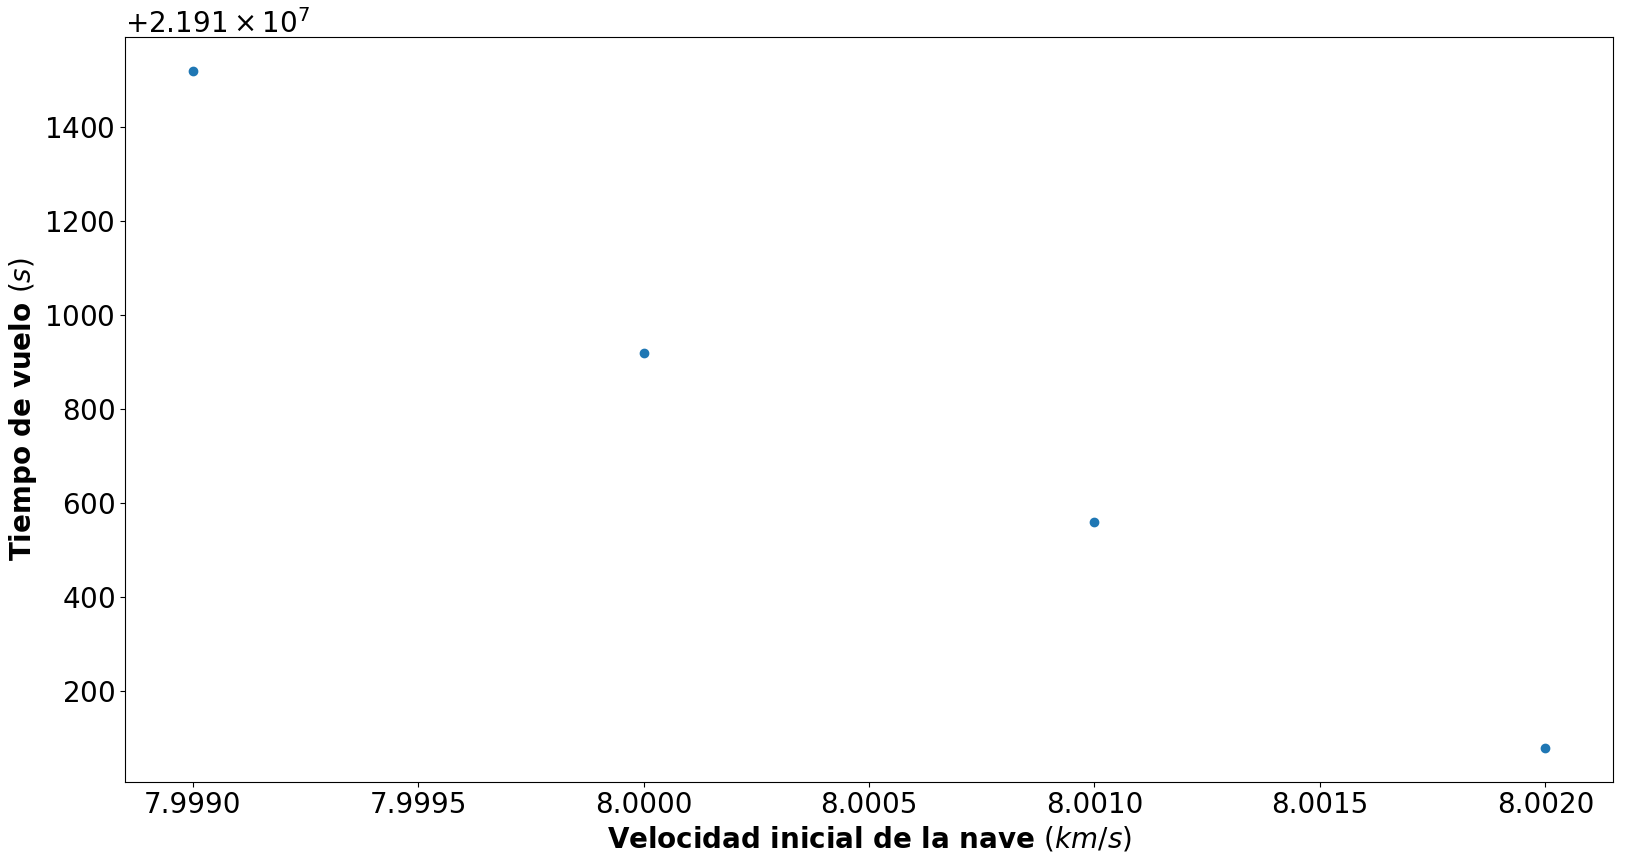
\includegraphics[width=0.9\textwidth]{./time_vs_v0_for_v_less_10^4_scatter}
                    \label{fig:marte_11}
                \end{figure}
                \begin{beamercolorbox}[sep=5pt,center]{block body}
                    \centering
                    \small{$\Delta t = 60s$ ; Misión exitosa si $d_{nave-marte} < 10^4 km$}
                \end{beamercolorbox}
            \end{frame}

        \subsection{Sistema con Júpiter}

            \begin{frame}{Animación del sistema}{}
                \vspace*{-0.3cm}
                \begin{minipage}[t]{0.49\textwidth}
                    \begin{figure}[H!]
                        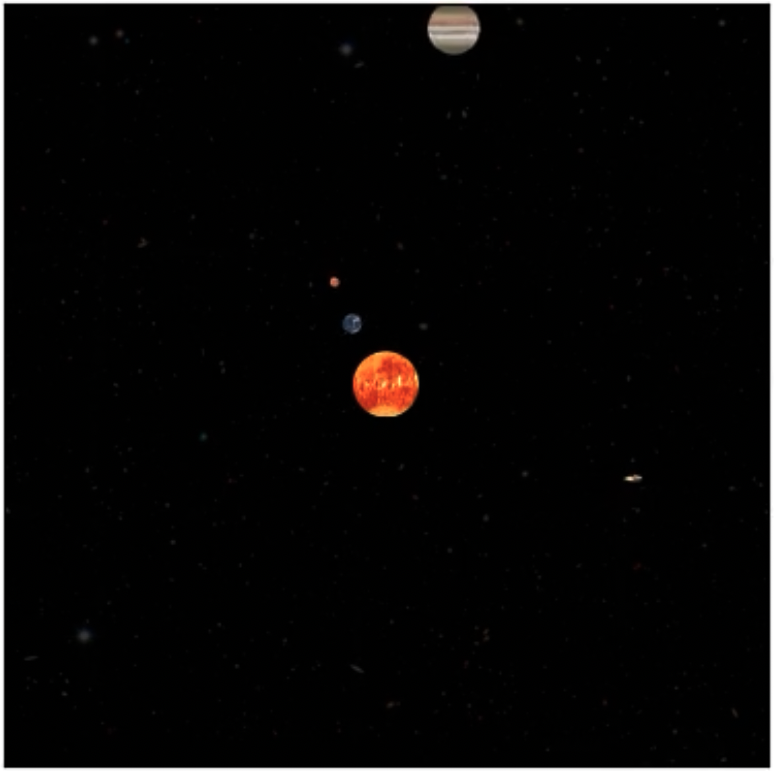
\includegraphics[width=\textwidth]{./animacion_jupiter_1}
                        \caption*{Véase la animación completa en \url{https://youtu.be/uGcs41rDAmk}.}
                        \label{fig:jupiter_1}
                    \end{figure}
                    \vspace*{-0.5cm}
                    \begin{beamercolorbox}[sep=5pt,center]{block body}
                        \centering
                        \small{Día de partida: 0}
                    \end{beamercolorbox}
                \end{minipage}
                \hfill
                \begin{minipage}[t]{0.49\textwidth}
                    \begin{figure}[H!]
                        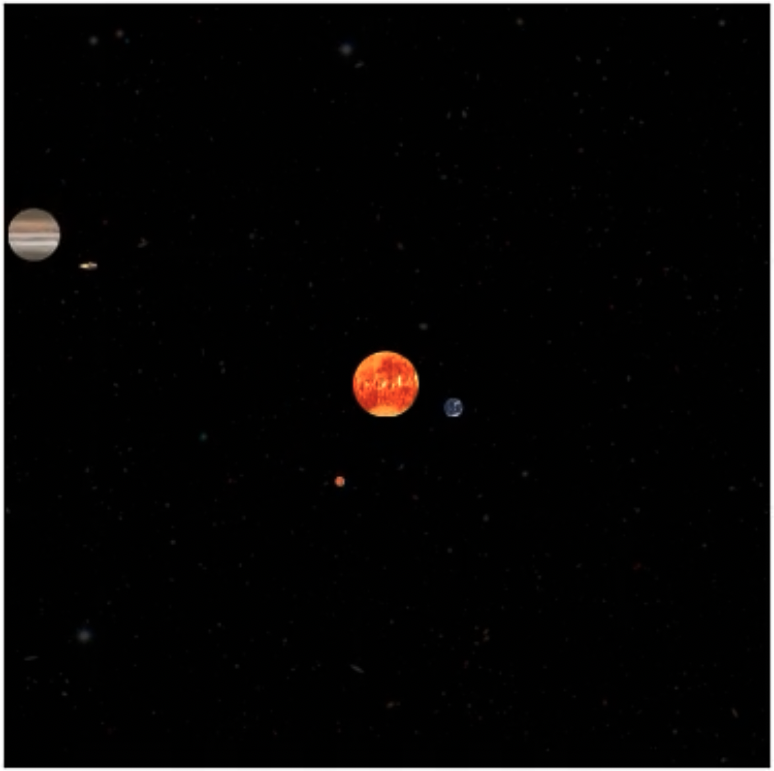
\includegraphics[width=\textwidth]{./animacion_jupiter_2}
                        \caption*{Véase la animación completa en \url{https://youtu.be/GijCuivfah8}.}
                        \label{fig:jupiter_2}
                    \end{figure}
                    \vspace*{-0.5cm}
                    \begin{beamercolorbox}[sep=5pt,center]{block body}
                        \centering
                        \small{Día de partida: 896}
                    \end{beamercolorbox}
                \end{minipage}
            \end{frame}

            \begin{frame}{Distancia mínima a Júpiter vs día de partida}{Momento óptimo de partida para arribar a Júpiter}
                \begin{figure}[H!]
                    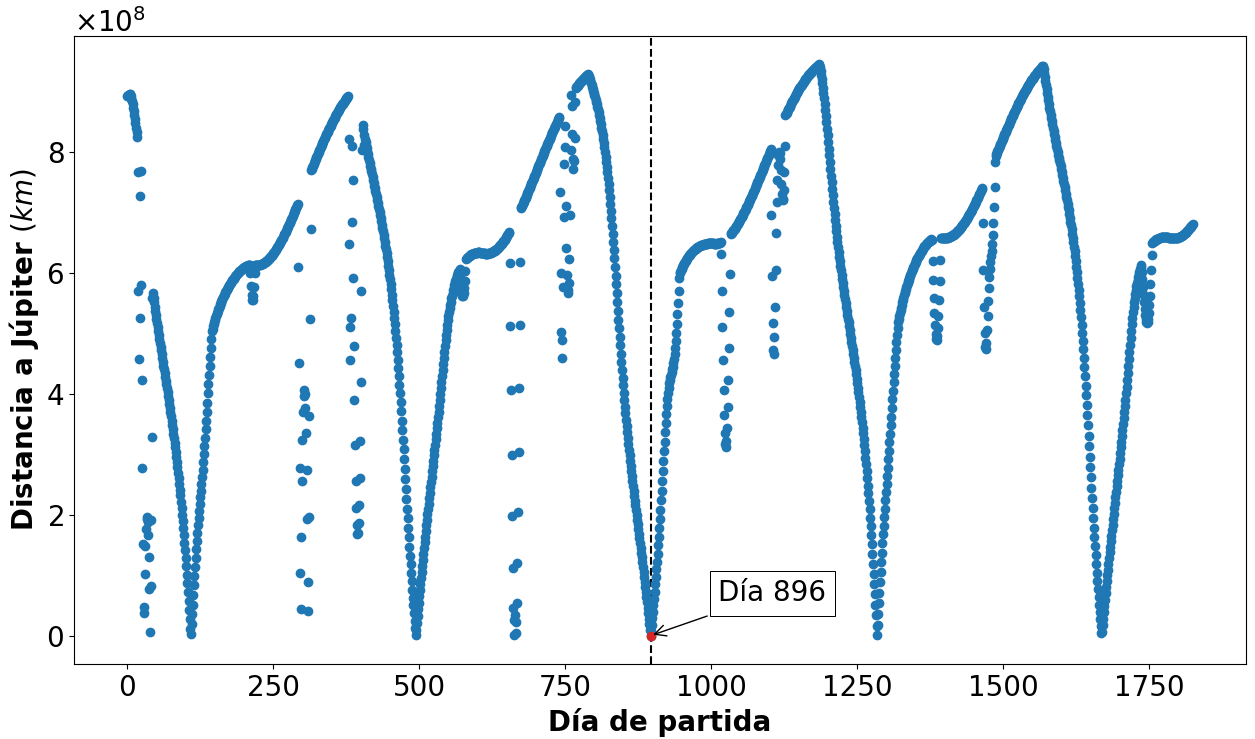
\includegraphics[width=0.9\textwidth]{./distancia_a_jupiter_vs_dia_de_partida}
                    \label{fig:jupiter_3}
                \end{figure}
                \begin{beamercolorbox}[sep=5pt,center]{block body}
                    \centering
                    \small{$\Delta t = 60s$ ; Misión exitosa si $d_{nave-jupiter} < 71000 km$}
                \end{beamercolorbox}
            \end{frame}

            \begin{frame}{Distancia mínima a Júpiter vs hora de partida}{Momento óptimo de partida para arribar a Júpiter. A partir de 895d}
                \begin{figure}[H!]
                    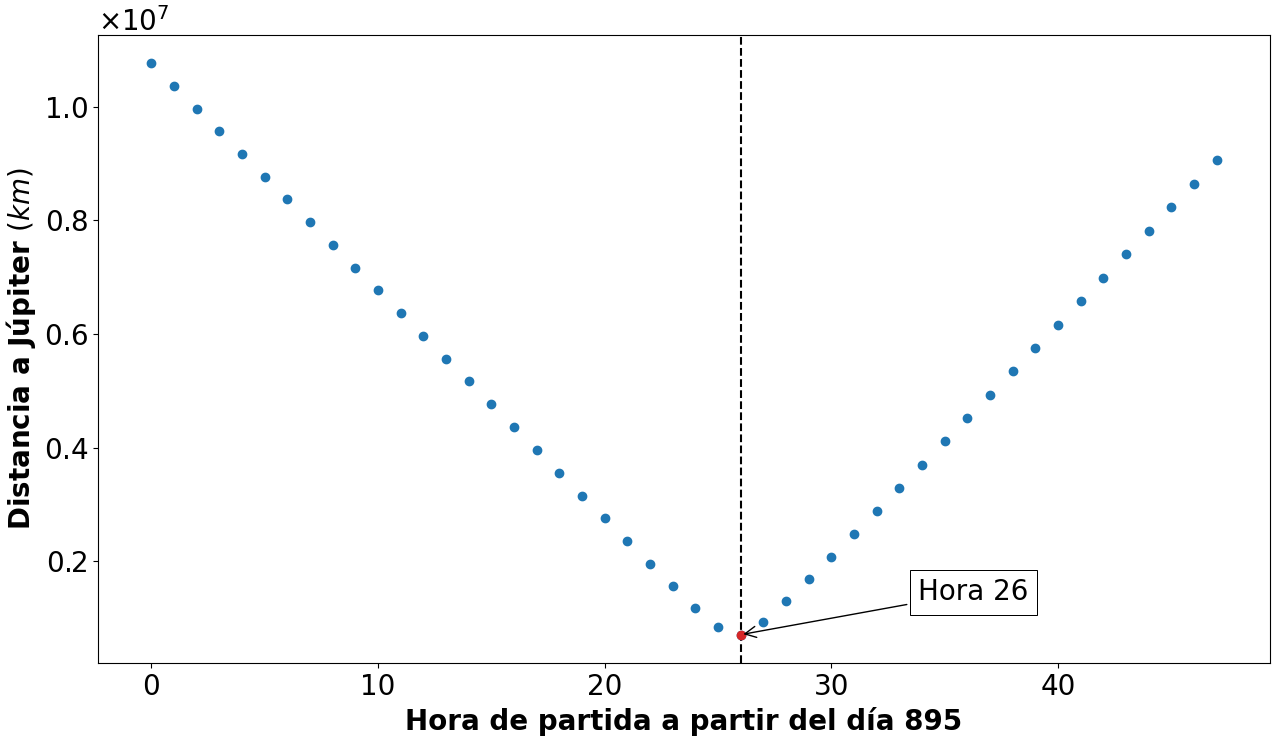
\includegraphics[width=0.9\textwidth]{./distancia_a_jupiter_vs_hora_de_partida}
                    \label{fig:jupiter_4}
                \end{figure}
                \begin{beamercolorbox}[sep=5pt,center]{block body}
                    \centering
                    \small{$\Delta t = 60s$ ; Misión exitosa si $d_{nave-jupiter} < 71000 km$}
                \end{beamercolorbox}
            \end{frame}

            \begin{frame}{Distancia mínima a Júpiter vs minuto de partida}{Momento óptimo de partida para arribar a Júpiter. A partir de 896d 1h}
                \begin{figure}[H!]
                    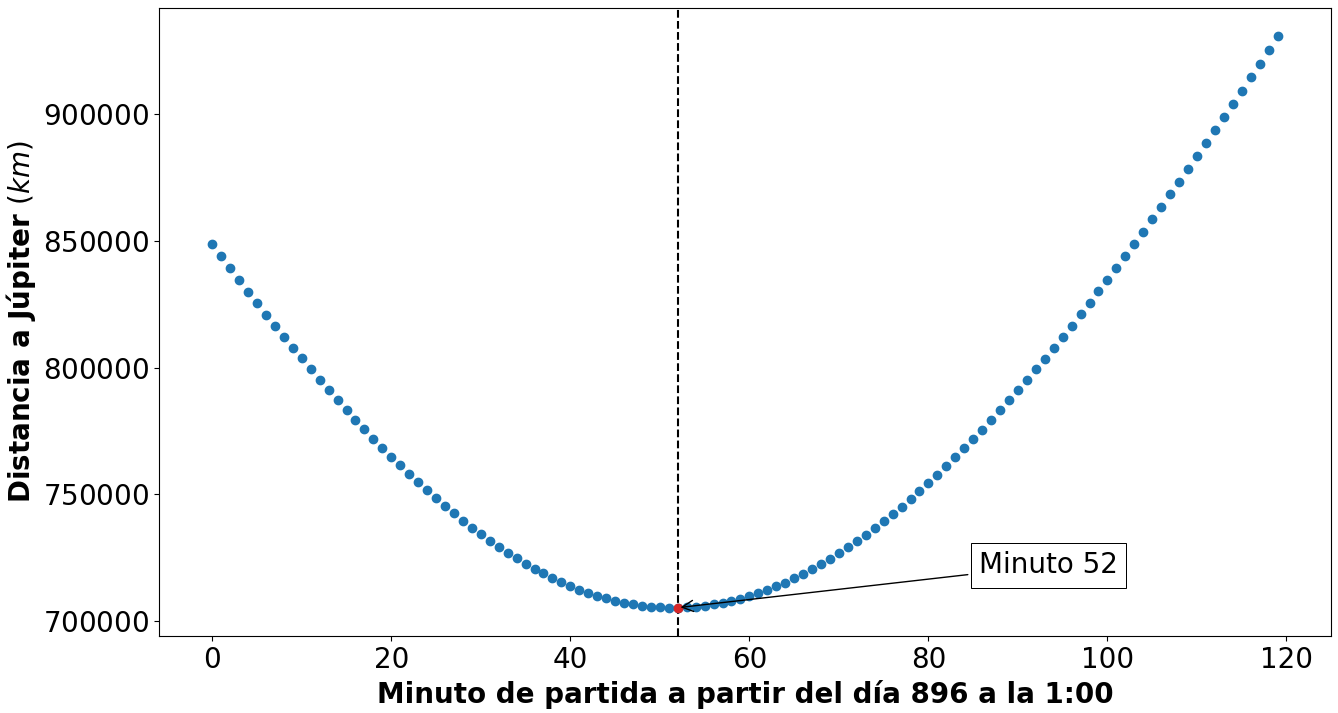
\includegraphics[width=0.9\textwidth]{./distancia_a_jupiter_vs_minuto_de_partida}
                    \label{fig:jupiter_5}
                \end{figure}
                \begin{beamercolorbox}[sep=5pt,center]{block body}
                    \centering
                    \small{$\Delta t = 60s$ ; $d_{nave-jupiter} = 705125 km$}
                \end{beamercolorbox}
            \end{frame}

            \begin{frame}{Distancia mínima a Júpiter vs velocidad inicial de la nave}{Partida de la nave: 896d 1h 52m}
                \begin{figure}[H!]
                    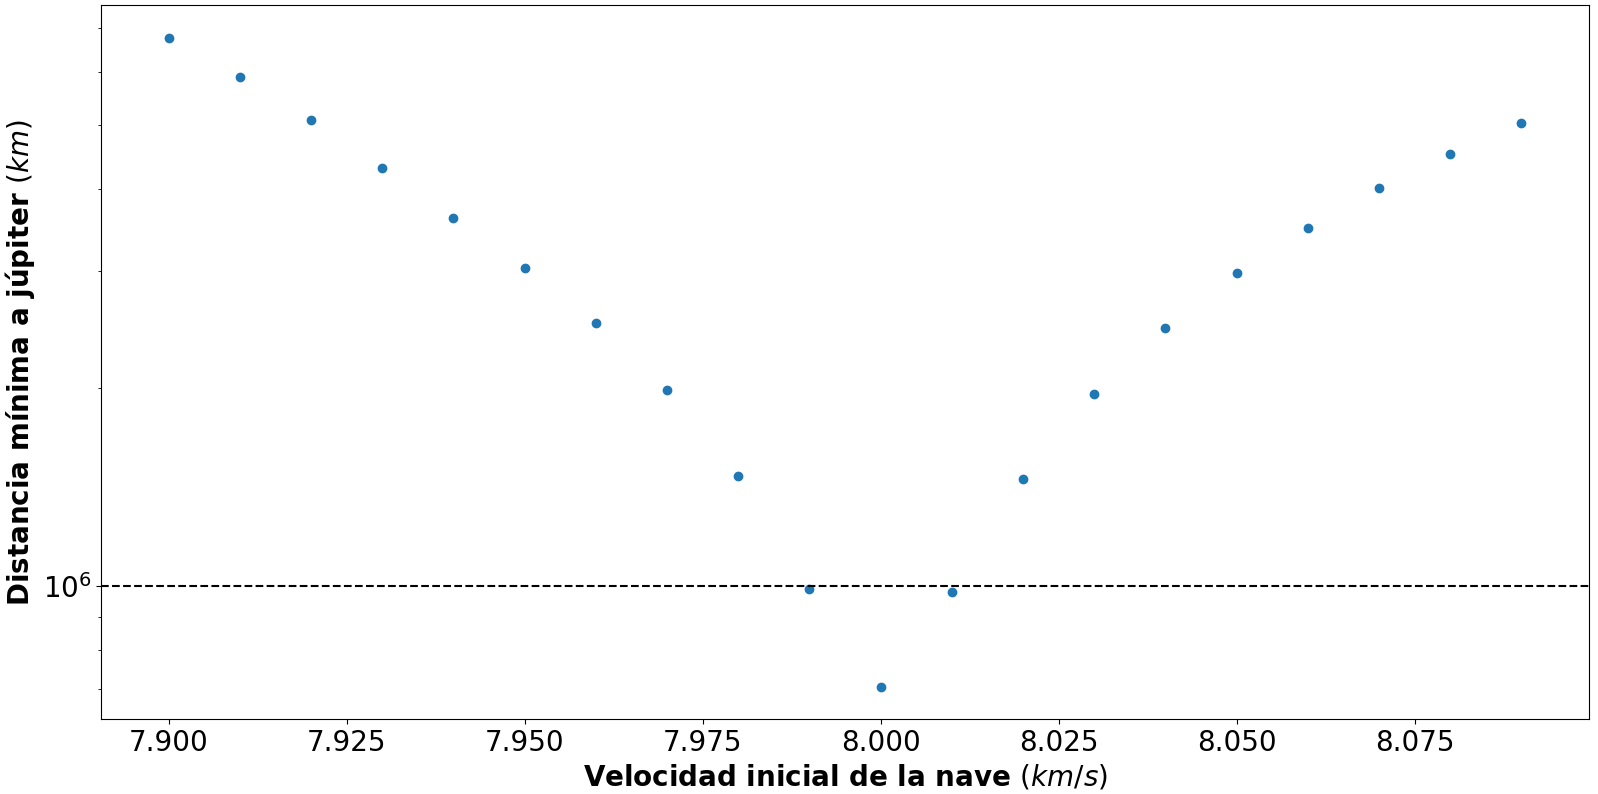
\includegraphics[width=0.9\textwidth]{./min_distance_vs_v0_logarithmic_jupiter}
                    \label{fig:jupiter_6}
                \end{figure}
                \begin{beamercolorbox}[sep=5pt,center]{block body}
                    \centering
                    \small{$\Delta t = 60s$ ; Misión exitosa si $d_{nave-jupiter} < 10^6 km$}
                \end{beamercolorbox}
            \end{frame}

            \begin{frame}{Tiempo de vuelo vs velocidad inicial de la nave}{Partida de la nave: 896d 1h 52m}
                \begin{figure}[H!]
                    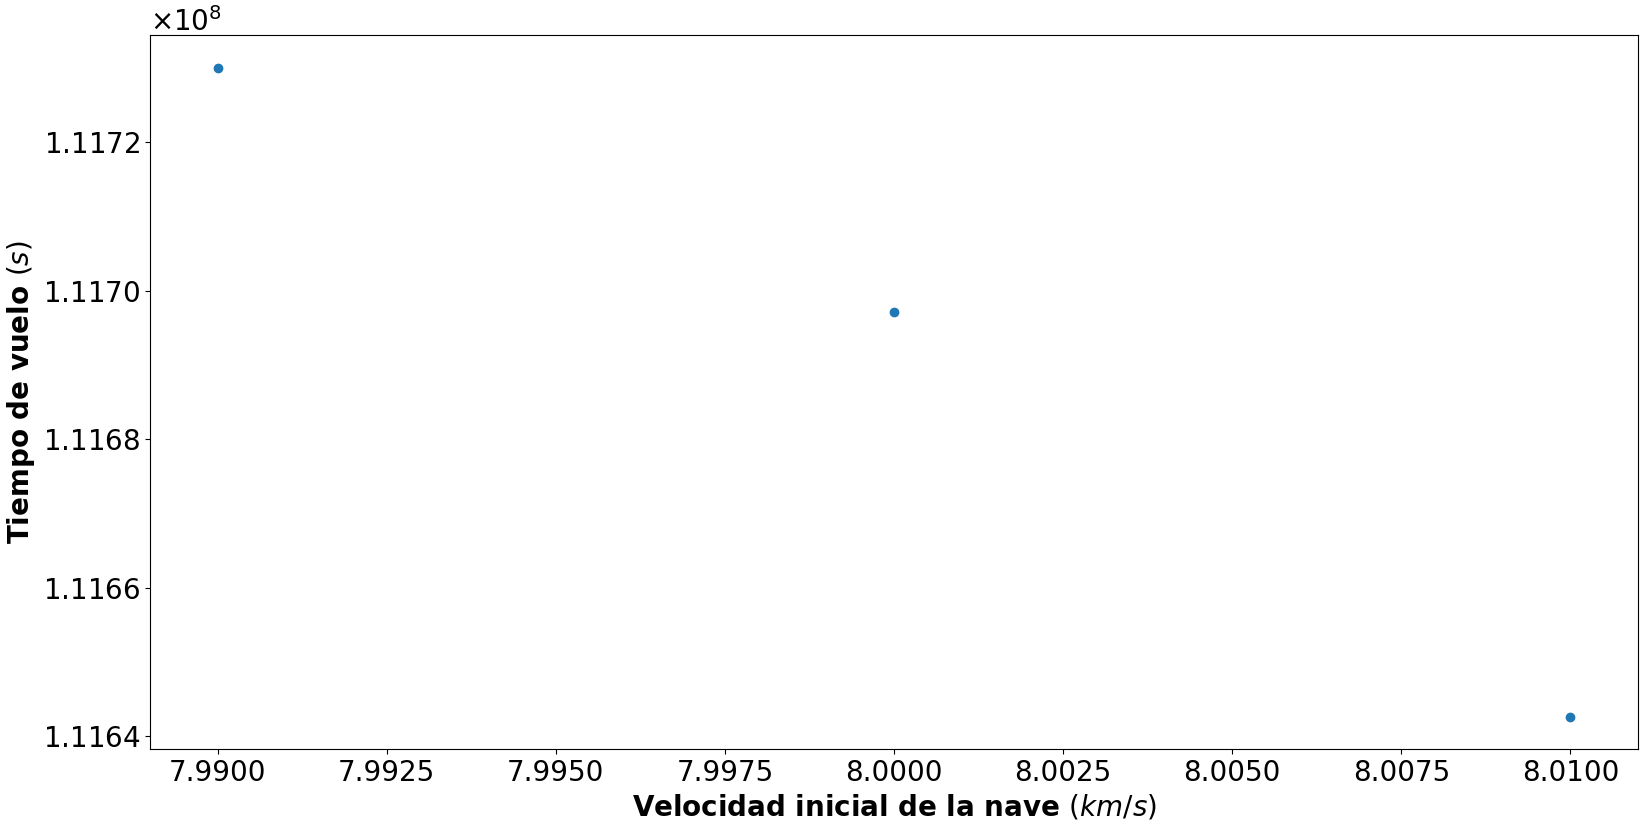
\includegraphics[width=0.9\textwidth]{./travel_time_vs_v0_logarithmic_jupiter}
                    \label{fig:jupiter_7}
                \end{figure}
                \begin{beamercolorbox}[sep=5pt,center]{block body}
                    \centering
                    \small{$\Delta t = 60s$ ; Misión exitosa si $d_{nave-jupiter} < 10^6 km$}
                \end{beamercolorbox}
            \end{frame}

    \section{Conclusiones}

        \begin{frame}{Conclusiones}
            \begin{itemize}
                \item El óptimo $\Delta t$ tiene un mínimo.
                Llega un punto que si se sigue disminuyendo, el error es mayor.
                \item Los cambios en la velocidad inicial de la nave resultan en una mayor distancia mínima a Marte.
                \item A medida que la nave se aleja del sol, su aceleración disminuye.
                \item Estas observaciones se pueden extrapolar a otros sistemas planetarios.
            \end{itemize}
        \end{frame}

        \begin{frame}
            \begin{beamercolorbox}[sep=8pt,center]{title}
                \usebeamerfont{title}{¡Muchas gracias!}
            \end{beamercolorbox}
        \end{frame}

\end{document}
